\chapter{Getting Started}

\section{Documentation Conventions}

Items to be selected from a menu are displayed in \menustyle{monospace font}.

Multilevel menu paths are separated by a / character. For example, \menustyle{Attenuation / 1x} means to open the
\menustyle{Attenuation} submenu and select the \menustyle{1x} item.

If there are multiple options for a menu or configuration option, they are displayed in square brackets and separated
by a | character. For example, \menustyle{Move waveform to / Waveform Group [1|2]} means to select either
\menustyle{Waveform Group 1} or \menustyle{Waveform Group 2} from the \menustyle{Move waveform to}
menu.

This project is under active development and is not anywhere near feature complete! As a result, this document is
likely to refer to active bug or feature request tickets on the GitHub issue trackers. Issues are referenced as
repository:ticket, for example scopehal-apps:3.

\section{Host System Requirements}

All current development is performed on Linux operating systems (primarily Debian and Arch), although experimental (and
incomplete) Windows support is provided. glscopeclient uses gtkmm as the UI toolkit. Current development mostly uses
3.24 but any recent 3.x version should work.

Any 64-bit ARM or Intel processor should be able to run glscopeclient. TODO: suggested minimum performance depending on
waveform depth etc?

A mouse with scroll wheel, or touchpad with scroll gesture support, is mandatory to enable full use of the UI. We may
explore alternative input methods for some UI elements in the future.

Waveform rendering is performed in compute shaders, so OpenGL 4.3 or newer is required as well as the
GL\_ARB\_gpu\_shader\_int64 extension. The corresponding minimum hardware requirement is an AMD Radeon HD 5000, NVIDIA
GeForce 400 series discrete GPU, or Intel Broadwell or newer integrated GPU plus suitably up-to-date drivers.
TODO: what AMD integrated/ARM GPUs started supporting GL 4.3?

To check for necessary graphics card support on Linux:
\begin{lstlisting}[language=sh]
glxinfo | grep GL_ARB_gpu_shader_int64
glxinfo | grep "OpenGL version string"
\end{lstlisting}

The minimum RAM requirement to actually launch glscopeclient is relatively small (TODO: do some testing) however
history mode and deep captures can easily consume many GB of RAM. We suggest 8GB as a reasonable minimum, with 32 or
more encouraged for deep history.

\section{Instrument Support}

glscopeclient uses the libscopehal library to communicate with oscilloscopes, so any libscopehal-compatible hardware
should work with glscopeclient. See the \hyperref[sec:drivers]{Oscilloscope Drivers} section for more details on which
hardware is supported and how to configure specific drivers.

\section{Compilation}

glscopeclient can be compiled on both Linux and Windows, but the specific steps that have to be taken differ quite a
lot between these the two.

\subsection{Linux}
\begin{enumerate}

\item Install dependencies. On Debian/Ubuntu:
\begin{lstlisting}[language=sh]
sudo apt install build-essential cmake pkg-config libglm-dev \
	libgtkmm-3.0-dev libsigc++-2.0-dev libyaml-cpp-dev \
	liblxi-dev texlive texlive-fonts-extra libglew-dev
\end{lstlisting}

\item Install FFTS library
\begin{lstlisting}[language=sh]
git clone https://github.com/anthonix/ffts.git
cd ffts
mkdir build
cd build
cmake ../
make -j4
sudo make install
\end{lstlisting}

\item Build scopehal and scopehal-apps
\begin{lstlisting}[language=sh]
git clone https://github.com/azonenberg/scopehal-apps.git --recurse-submodules
cd scopehal-apps
mkdir build
cd build
cmake ../
make -j4
\end{lstlisting}

\item Install scopehal and scopehal-apps: right now, you don't. As of now, glscopeclient is intended to be run from the
glscopeclient source directory (src/glscopeclient). Anybody want to contribute and set up a proper install process?

\end{enumerate}

\subsection{Windows}

On Windows, we make use of the MSYS2 development environment, which gives us access to the MingGW-w64 toolchain. Since this toolchain allows glscopeclient to be compiled as a native Windows application, MSYS2 is only needed to actually compile the project, not to run it.

\begin{enumerate}

\item Download and install MSYS2. You can download it here: \url{https://www.msys2.org/}\\
It is of utmost importance that \textbf{all} steps outlined on the website are followed precisely, even if they might seem unnecessary. This will avoid lots of hard to diagnose problems later on in the build.\\

All following steps are to be done in a MinGW64 shell (\textbf{not} in a MSYS shell, which also gets installed by the MSYS2 installer).

\item Install build tools
\begin{lstlisting}[language=sh]
pacman -S mingw-w64-x86_64-gcc mingw-w64-x86_64-cmake \
    mingw-w64-x86_64-make
\end{lstlisting}

\item Install dependencies
\begin{lstlisting}[language=sh]
pacman -S mingw-w64-x86_64-glm mingw-w64-x86_64-libsigc++ \
    mingw-w64-x86_64-gtkmm3 mingw-w64-x86_64-yaml-cpp \
    mingw-w64-x86_64-glew
\end{lstlisting}

\item Build FFTS library
\begin{lstlisting}[language=sh]
git clone https://github.com/anthonix/ffts.git
cd ffts
mkdir build
cd build
cmake -G"MinGW Makefiles" -DCMAKE_INSTALL_PREFIX=$MSYSTEM_PREFIX ..
mingw32-make -j4
mingw32-make install
\end{lstlisting}

\item Build scopehal and scopehal-apps
\begin{lstlisting}[language=sh]
git clone https://github.com/azonenberg/scopehal-apps.git --recurse-submodules
cd scopehal-apps
mkdir build
cd build
cmake -G"MinGW Makefiles" -DLIBFFTS_INCLUDE_DIR=/mingw64/include/ \
    -DLIBFFTS_LIBRARIES=/mingw64/lib/libffts_static.a ./..
mingw32-make -j4
\end{lstlisting}

\item Copying binaries and running glscopeclient \\
Since glscopeclient is built using the MinGW toolchain, it depends on a rather large number of dynamic libraries. Since the application cannot find these libraries when being run from the build directory, there are two ways to make glscopeclient runnable: ``packaging'' the application by collecting all the depedencies, and installing it into the MinGW64 virtual file system.

\begin{enumerate}
\item Installing glscopeclient into the virtual filesystem
\begin{lstlisting}[language=sh]
cp ./src/glscopeclient/glscopeclient.exe /mingw64/bin/
cp -r ./src/glscopeclient/shaders /mingw64/bin/
cp -r ./src/glscopeclient/styles /mingw64/bin/
cp -r ./src/glscopeclient/gradients /mingw64/bin/
cp ./lib/graphwidget/libgraphwidget.dll /mingw64/bin/
cp ./lib/log/liblog.dll /mingw64/bin/
cp ./lib/scopehal/libscopehal.dll /mingw64/bin/
cp ./lib/scopeprotocols/libscopeprotocols.dll /mingw64/bin/
\end{lstlisting}
\vspace{0.5cm}
The application can now be started from any MinGW64 terminal session:
\vspace{0.5cm}
\begin{lstlisting}[language=sh]
glscopeclient.exe
\end{lstlisting}
\vspace{0.5cm}

\item Packaging glscopeclient and its depedencies
This approach is not officially supported yet.
\end{enumerate}

\end{enumerate}


\section{Running glscopeclient}

When running glscopeclient with no arguments, a dialog box (Fig. \ref{connection-dialog}) is displayed allowing you to
connect to an instrument. As of this writing, there is no support for connecting to multiple instruments via the
dialog.

\begin{figure}[h]
\centering
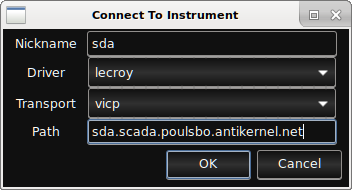
\includegraphics[width=6cm]{images/connection-dialog.png}
\caption{Connection dialog}
\label{connection-dialog}
\end{figure}

It is also possible to connect to arbitrarily many instruments by passing the ``connection string" for each instrument
as a command-line argument.

\begin{lstlisting}[language=sh]
./glscopeclient --debug \
	mylecroy:lecroy:vicp:myscope.example.com:1234 \
	myrigol:rigol:lan:rigol.example.com
\end{lstlisting}

The \texttt{--debug} argument may be omitted or replaced with any other liblogtools argument for controlling console
debug verbosity (\texttt{--quiet}, \texttt{--verbose}, \texttt{--debug}, \texttt{--trace}, etc). If you're using
glscopeclient at its current level of maturity you're probably a developer, so we suggest \texttt{--debug} by default.

Each instrument is described by a ``connection string" containing four colon-separated fields.

\begin{itemize}
\item Nickname. This can be any text string not containing spaces or colons. If you have only one instrument it's
largely ignored, but when multiple instruments are present channel names in the UI are prefixed with the nickname to
avoid ambiguity.
\item Driver name. This is a string identifying the command protocol the scope uses. Note that not all
scopes from the same vendor will use the same command set or driver!
\item Transport. This is is a string describing how the driver connects to the scope (e.g. RS232 or Ethernet)
\item Arguments for the driver identifying the device to connect to, separated by colons. This varies by driver but is
typically a hostname:port combination, TTY device path, or similar.
\end{itemize}

Some users have reported better performance by setting the OMP\_WAIT\_POLICY environment variable to PASSIVE.

\section{Design Philosophy}

glscopeclient's UI is heavily mouse driven and context based. Space used by always-visible buttons, sliders, etc is
kept to a minimum in order to keep as much screen real estate as possible usable for waveform display. Additional
controls are displayed in menus or pop-up dialogs, then hidden as soon as they are not needed.

Most UI elements can be interacted with by left clicking (select), left dragging (move), using the scroll wheel (zoom),
double clicking (open properties dialog), or right clicking (context menu).

Most text fields allow SI prefixes for scaling values (mV, us, GHz, etc).
